\subsection{The Third Refinement}
\label{sec:component_diagrams-tutorial_thirdRefinement}

 
 
Now we refine the notion of the Program. We associate with each PID a washTime, rinseTime and spinTime and also introduce a WashCount and SpinCount as shown in Figure \ref{fig:AddingWashProgramDetailsToTheModel}. These properties constrain and make deterministic the operation of the washing machine sub-system for a given PID.
 
 \begin{figure}[!htbp]
  \centering
  \ifplastex
  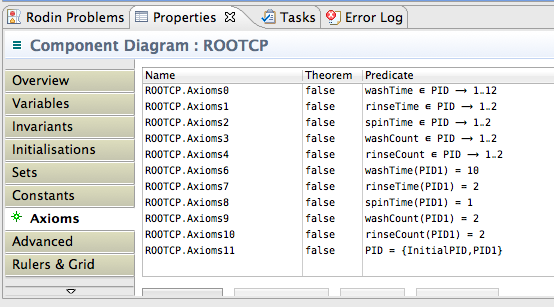
\includegraphics[width=1024]{figures/image36.png}
  \else
  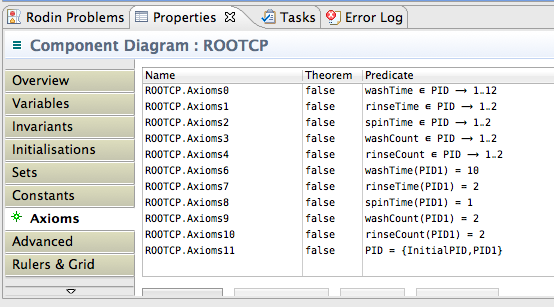
\includegraphics[width=1\textwidth]{figures/image36.png}
  \fi
  \caption{Adding Wash Program Details to the Model}
  \label{fig:AddingWashProgramDetailsToTheModel}
\end{figure} 
 
The delay introduced for each wash mode is modelled using a SelfWake as shown for the rinse mode in Figure \ref{fig:IntroducingWashProgramDelaysUsingSelfWakes}.
 
 \begin{figure}[!htbp]
  \centering
  \ifplastex
  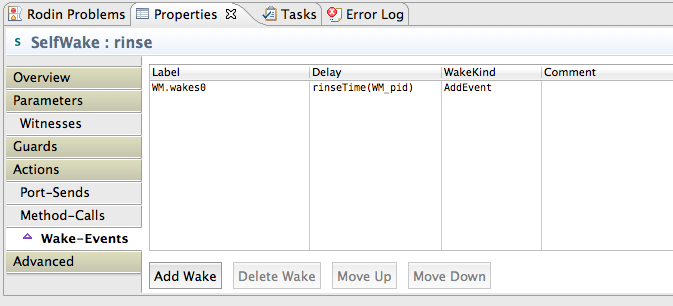
\includegraphics[width=1024]{figures/image37.png}
  \else
  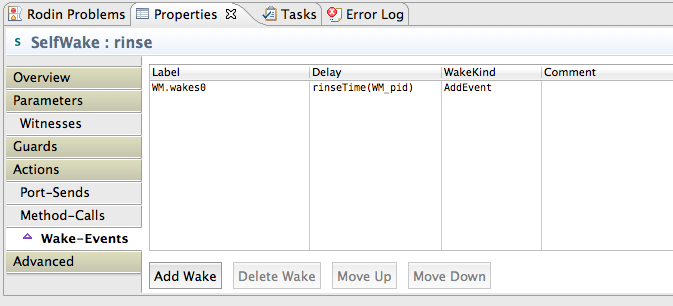
\includegraphics[width=1\textwidth]{figures/image37.png}
  \fi
  \caption{Introducing Wash Program Delays using Self Wakes}
  \label{fig:IntroducingWashProgramDelaysUsingSelfWakes}
\end{figure} 

 
The number of washes or rinses associated with a program is modelled using a counter which is decremented and hence completes at rinseCounter = 0, as shown in Figure \ref{fig:IntroducingWashProgramCyclesUsingGuards}.
 
 \begin{figure}[!htbp]
  \centering
  \ifplastex
  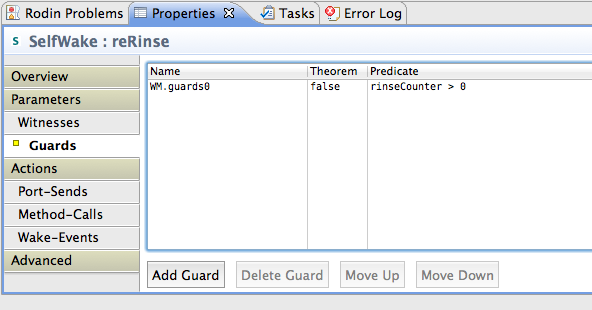
\includegraphics[width=1024]{figures/image38.png}
  \else
  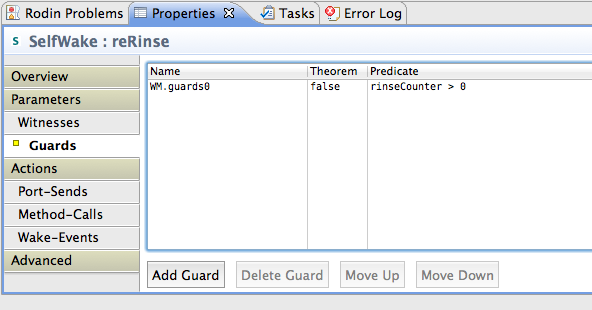
\includegraphics[width=1\textwidth]{figures/image38.png}
  \fi
  \caption{Introducing Wash Program Cycles using Guards}
  \label{fig:IntroducingWashProgramCyclesUsingGuards}
\end{figure} 
 
Again, the model checker is run to verify that no deadlocks have been introduced into the system. Since this refinement is only to strengthen the guards, invariant preservation is not an issue in this refinement. Note that as shown in Figure \ref{fig:ProBModelCheckingCoverageForTheThirdRefinement}, full operation coverage is achieved. The program constraints introduced in this refinement have reduced the model state space. 
 
 \begin{figure}[!htbp]
  \centering
  \ifplastex
  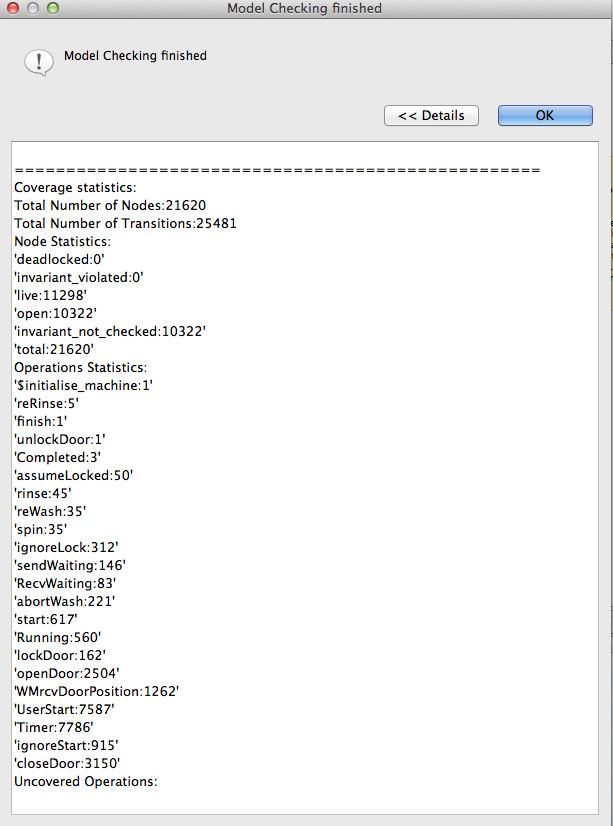
\includegraphics[width=1024]{figures/image39.png}
  \else
  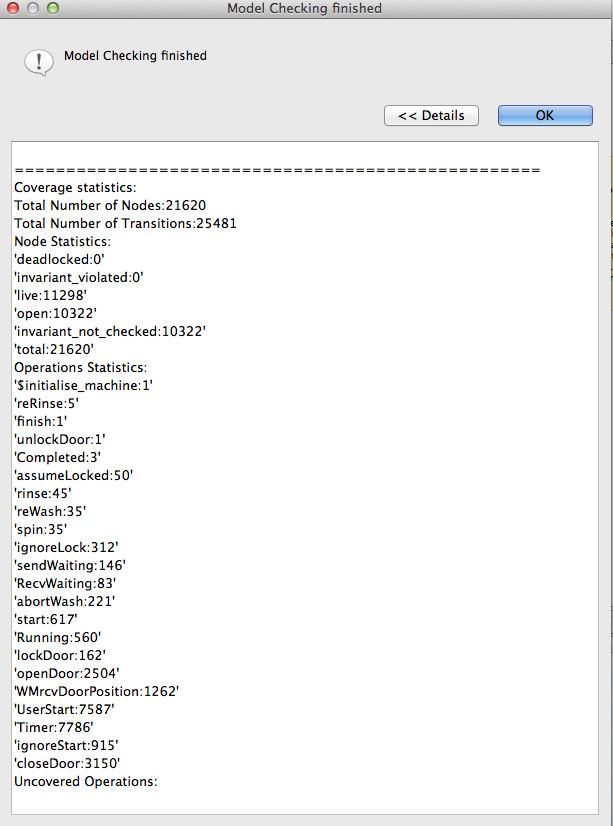
\includegraphics[width=1\textwidth]{figures/image39.png}
  \fi
  \caption{ProB Model Checking Coverage for the Third Refinement}
  \label{fig:ProBModelCheckingCoverageForTheThirdRefinement}
\end{figure} 
 
The state machine is shown in Figure \ref{fig:StatemachineForTheThirdRefinement} below. Invariants concerning the counters have been added to the INPROGRESS and RINSING states. These invariants help ensure that no mistakes have been made in constructing the counters.
 
 \begin{figure}[!htbp]
  \centering
  \ifplastex
  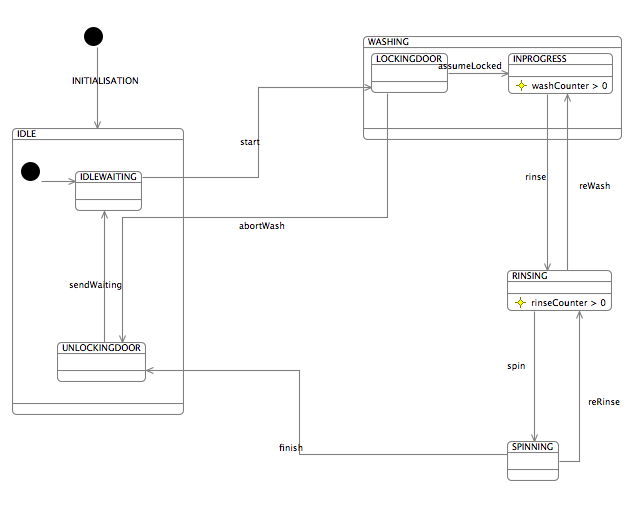
\includegraphics[width=1024]{figures/image40.png}
  \else
  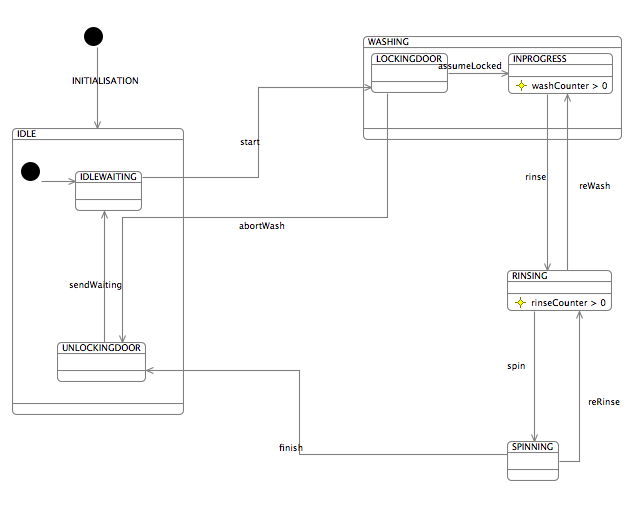
\includegraphics[width=1\textwidth]{figures/image40.png}
  \fi
  \caption{State-machine for the Third Refinement }
  \label{fig:StatemachineForTheThirdRefinement}
\end{figure} 
 

%%% Local Variables:
%%% mode: latex
%%% TeX-master: "component_diagrams-user_manual"
%%% End:
